\documentclass[letterpaper]{article}
\usepackage{settings}

\begin{document}
\begin{notes}{Part 6: Storage and Compression}

\NoteChapter{Image Storage and File Formats}

Long before JPEG and PNG, storing an image on a computer required solving a deceptively hard problem: how do you encode a 2D grid of color values as a flat sequence of bytes? The answer evolved over four decades, driven by hardware constraints, commercial incentives, and the gradual discovery that most image data is highly redundant.

\NoteSection{The First Digital Images}


\begin{figure}[H]
    \centering
    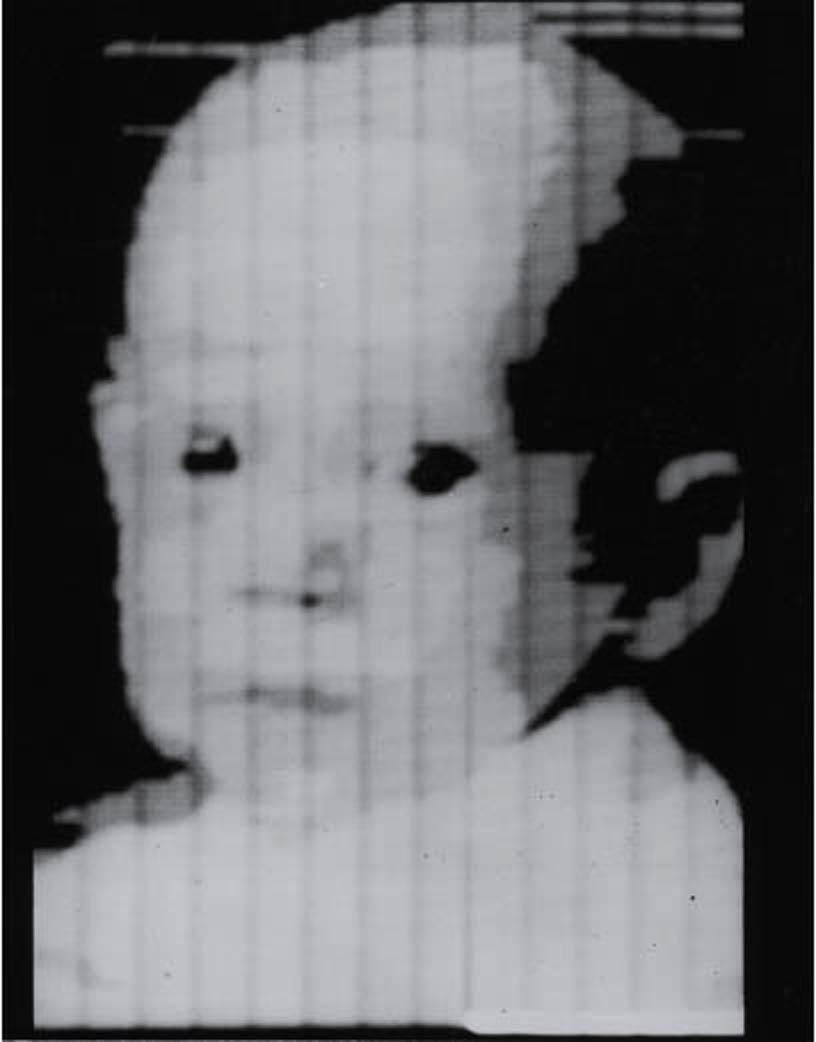
\includegraphics[width=0.5\linewidth]{images/part6/first-digital-image.png}
    \caption{The first digital image, created in 1957 with a rotating-drum scanner, first invented by NIST.}
\end{figure}

\textbf{Facsimile and raster scanning (1920s--1950s).} The concept of raster scanning --- decomposing a 2D image into a sequence of rows, each row into discrete samples --- predates computers entirely. The Bartlane cable picture transmission system (1921) sent newspaper photographs across the Atlantic via telegraph by encoding each pixel as one of five discrete brightness levels. The first image digitized on an actual computer was a photograph of Russell Kirsch's infant son, scanned in 1957 on the SEAC computer at the National Bureau of Standards at a resolution of $176\times176$ pixels, 1 bit per pixel.\\

\textbf{Video display memory and the framebuffer (1960s--1970s).} Early computers had no dedicated display hardware. Images lived in core memory and were sent line by line to a raster-scan CRT. The entire image in memory is called a \emph{framebuffer}. Each bit (or small group of bits) in the framebuffer corresponded directly to one pixel on screen: display hardware scanned through the buffer at a fixed rate synchronized to the CRT beam, converting integer values to analog voltages. The ``resolution'' of the image was therefore dictated entirely by how much memory the machine could afford to dedicate.

\NoteSection{Bit Depth and Color Representation}

\textbf{Bit depth} is the number of bits allocated per pixel. It determines the maximum number of distinct values (intensity levels or color indices) a pixel can take: $2^b$ values for $b$ bits.\\

\textbf{1-bit (monochrome).} Each pixel is 0 (black) or 1 (white). Eight pixels are packed into one byte. A $640\times480$ binary image occupies $640\times480/8 = 38{,}400$ bytes $\approx 37.5\,\text{KB}$. Used for facsimile (ITU-T T.4/T.6 Group 3/4), text rendering, early laser printers, and the first computer graphics terminals.


\begin{figure}[H]
    \centering
    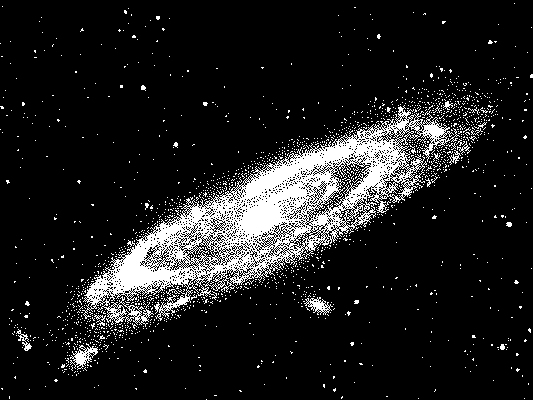
\includegraphics[width=0.5\linewidth]{images/part6/1-bit-image.png}
    \caption{A one-bit image}
\end{figure}

\textbf{4-bit (16 colors).} Used in IBM CGA (1981) and EGA (1984) display adapters. Each byte stores two pixels in its upper and lower nibbles. The value 0--15 is an index into a fixed hardware palette of 16 colors. A $320\times200$ CGA screen required $320\times200\times4/8=32{,}000$ bytes of framebuffer.\\

\textbf{8-bit indexed color.} The dominant standard of the late 1980s and early 1990s (VGA mode 13h, SVGA). Each pixel is one byte (0--255) that indexes into a \emph{color look-up table} (CLUT) of 256 RGB triples. The CLUT itself requires $256\times3=768$ bytes. A $640\times480$ image is $307{,}200$ bytes $\approx 300\,\text{KB}$ of pixel data plus the palette. GIF (1987) is built entirely on this model.\\

\textbf{16-bit high color.} Two bytes per pixel. The most common packing is \emph{5-6-5 RGB}: 5 bits for red, 6 for green (the human eye has highest green sensitivity), 5 for blue. Alternatively \emph{5-5-5} with one unused bit, or \emph{5-5-5-1} with 1-bit alpha. Popularized by VESA SVGA modes in the early 1990s and still common in embedded framebuffers today.\\

\textbf{24-bit true color.} Three bytes per pixel, one each for R, G, B. Yields $2^{24}=16{,}777{,}216$ distinct colors --- far more than the human visual system can discriminate. A $640\times480$ true-color image occupies $640\times480\times3=921{,}600$ bytes $\approx 900\,\text{KB}$. BMP (1986) supports 24-bit natively; JPEG (1992) targets this color space.\\

\textbf{32-bit (RGBA).} Four bytes per pixel, adding an 8-bit alpha channel for per-pixel transparency. The extra byte is often worth keeping even when alpha is unused because 32-bit-aligned accesses are faster on hardware word boundaries.

\NoteSection{Color Look-Up Tables (CLUTs)}

A CLUT (also called a \emph{palette} or \emph{colormap}) separates pixel storage from color specification. The pixel array stores small integer \emph{indices}; a separate table maps each index to a full RGB triple.\\

\textbf{Advantages.} Drastic memory savings when the number of distinct colors is small. A $1024\times768$ image using at most 256 colors requires $1024\times768=786{,}432$ bytes of indices plus 768 bytes of palette, versus $1024\times768\times3=2{,}359{,}296$ bytes of 24-bit true color.\\

\textbf{Disadvantages.} Photographs contain far more than 256 colors, so palette-based storage requires first \emph{quantizing} the color space (median-cut, k-means) to select the 256 best representative colors, then replacing each pixel with its nearest palette entry. The resulting \emph{posterization} (visible color banding) is mitigated by \emph{dithering} (Floyd--Steinberg, ordered dither), which diffuses quantization error spatially at the cost of fine texture.

\NoteSection{Raw Raster Layout in Memory}

\textbf{Row-major (scanline) order.} The standard in-memory representation stores pixels row by row, left to right, top to bottom. For a $W\times H$ image with $d$ bytes per pixel, the byte offset of pixel $(x,y)$ is
$$\text{offset}(x,y)=y\cdot\text{stride}+x\cdot d,$$
where \emph{stride} (also called \emph{pitch}) is the number of bytes per scanline.\\

\textbf{Scanline padding.} Many formats require each scanline to begin on a memory-alignment boundary. BMP, for instance, pads every row to a multiple of 4 bytes:
$$\text{stride}=\left\lceil\frac{W\cdot d}{4}\right\rceil\times 4.$$

\textbf{Top-down vs.\ bottom-up.} BMP stores rows bottom-up (row 0 is the bottom row), a convention inherited from mathematical $(x,y)$ coordinates and early CRT raster conventions. Most other formats (PNG, JPEG, TIFF) store top-down.\\

\textbf{Planar vs.\ interleaved layout.} In \emph{interleaved} (packed pixel) format, all channels of a pixel are contiguous: RGBRGBRGB\ldots. In \emph{planar} format, each channel is a separate contiguous array: RRR\ldots GGG\ldots BBB\ldots. Interleaved is standard for display memory and most image files; planar is used in some video formats (YUV 4:2:0, I420) and multi-band remote-sensing data.

\NoteSection{Early Raster File Formats}

File formats add a header and optional metadata around the raw pixel array, allowing programs to correctly interpret bit depth, dimensions, and color model without out-of-band information.\\

\textbf{PBM / PGM / PPM (Netpbm, 1980s).} The simplest possible portable formats: ASCII or raw binary with a minimal header. A PBM file for a $W\times H$ binary image begins with the magic bytes \texttt{P1}, followed by width, height, and then $W\times H$ space-separated \texttt{0}/\texttt{1} values. PGM extends this to grayscale (up to 16 bits), PPM to 24-bit RGB. No compression. Still widely used for prototyping and unit tests because they need no library to read or write.\\

\textbf{PCX (ZSoft PC Paintbrush, 1984).} One of the first widespread PC image formats, shipped with PC Paintbrush. Supports 1-bit through 24-bit color and uses a simple per-scanline run-length encoding with a 2-bit tag byte. Superseded by more capable formats but still found in legacy CAD software and DOS-era games.\\

\textbf{TIFF (Aldus / Adobe, 1986).} Tagged Image File Format: a flexible container built around \emph{tags} (key--value pairs stored in an image file directory). Every property --- width, height, bit depth, color space, compression scheme --- is declared via a tag, making TIFF self-describing and extensible. Supported compression methods include none, PackBits RLE, LZW, CCITT Group 4 (fax), and later JPEG. Multi-page images and floating-point data are supported natively. TIFF remains the standard archival format in professional photography, medical imaging, and printing.\\

\textbf{BMP (Windows Device-Independent Bitmap, 1986).} The native raster format of Microsoft Windows, introduced with Windows 1.0. A BMP file consists of a 14-byte file header, a DIB header (BITMAPINFOHEADER and variants), an optional CLUT, and raw pixel data in padded bottom-up scanlines. Supports 1, 4, 8, 16, 24, and 32 bits per pixel with optional RLE compression for 4- and 8-bit images. Trivial to implement and still used as a Windows clipboard format and debugging target.\\

\textbf{GIF (CompuServe, 1987).} Graphics Interchange Format: the first widely deployed losslessly compressed image format on the Internet. Key design choices:
\begin{itemize}
    \item \emph{Indexed 8-bit color}: each pixel stores a palette index; at most 256 simultaneous colors per frame.
    \item \emph{LZW lossless compression}: each scanline is LZW-compressed (achieves 30--50\% size reduction for cartoon-style images).
    \item \emph{Transparency}: one palette index may be designated transparent (1-bit alpha).
    \item \emph{Animation (GIF89a, 1989)}: multiple frames with per-frame delays and disposal methods --- the origin of web animation.
\end{itemize}
The 256-color ceiling made GIF unsuitable for photographs but ideal for logos, icons, line art, and sprite graphics. Unisys's 1994 patent enforcement over the LZW algorithm motivated the creation of PNG (1996) as a patent-free, non-palette alternative.


\columnbreaknofill



\NoteChapter{Image Compression}


Image compression reduces the number of bits needed to store or transmit an image. Two fundamental limits govern how far compression can go:
\begin{itemize}
    \item \textbf{Shannon entropy} - the theoretical minimum bits per symbol for a lossless code: 
    $$H = -\sum_k p_k \log_2 p_k$$
    No lossless coder can beat this bound.
    \item \textbf{Rate--distortion trade-off} - for lossy coding, there is always a trade-off between bit-rate $R$ (bits per pixel) and distortion $D$ (e.g., MSE). The rate--distortion function $R(D)$ gives the minimum rate needed to achieve distortion $\le D$.
\end{itemize}

\textbf{Taxonomy.}
\begin{itemize}
    \item \emph{Lossless}: exact reconstruction; exploits statistical redundancy only. Examples: PNG, GIF, TIFF-LZW.
    \item \emph{Lossy}: discards information the human visual system (HVS) is insensitive to; achieves far higher compression ratios. Examples: JPEG, JPEG 2000, WebP, HEIC.
\end{itemize}

\textbf{Three types of redundancy} that all compression methods exploit:
\begin{enumerate}
    \item \emph{Coding redundancy}: some intensity values occur more often; assigning shorter codes to frequent values reduces average code length (Huffman, arithmetic coding).
    \item \emph{Spatial (interpixel) redundancy}: neighboring pixels are correlated; predicting each pixel from its neighbors and coding only the residual is efficient (run-length encoding, LZ, DCT decorrelation).
    \item \emph{Psychovisual redundancy}: the HVS is less sensitive to high spatial frequencies and to chrominance detail; quantising these heavily causes little perceived loss.
\end{enumerate}

\NoteSection{Lossless Compression}

\textbf{Run-Length Encoding (RLE).} Replace runs of identical values with (value, count) pairs. Effective for binary images or images with large flat regions; useless for natural photographs.\\

\textbf{Huffman Coding.} Assign variable-length prefix-free codes to symbols based on their probabilities. Build a binary tree bottom-up: repeatedly merge the two nodes with the smallest probability; the resulting code length for symbol $k$ is $\approx -\log_2 p_k$ bits. Optimal for integer-length codes; approaches Shannon entropy. Used inside JPEG and PNG.\\

\textbf{Arithmetic Coding.} Encodes an entire message as a single number in $[0,1)$, recursively subdividing the interval according to symbol probabilities. Achieves entropy to within 1 bit per message regardless of symbol probabilities - better than Huffman for highly skewed distributions. Computationally more expensive but used in JPEG 2000 (MQ coder) and modern video codecs.\\

\textbf{LZ77 / Deflate / PNG.} LZ-family coders replace repeated byte sequences with back-references (offset, length) into a sliding window of previous output. PNG uses Deflate (LZ77 + Huffman), preceded by a per-row \emph{prediction filter} (Sub, Up, Average, or Paeth) to decorrelate pixels before entropy coding. Completely lossless; PNG is the standard for screenshots, graphics, and medical images where exact values must be preserved.

\NoteSection{Transform Coding (Lossy Framework)}

Most practical lossy codecs share the same three-step framework:
\begin{enumerate}
    \item \textbf{Transform}: map the image (or a block) to a domain where energy is concentrated in a few coefficients. Uncorrelated coefficients can be quantised independently.
    \item \textbf{Quantise}: round each transform coefficient to a finite set of levels. This is the \emph{only lossy step} - it discards information irreversibly. Coarser quantisation $\Rightarrow$ more compression, more distortion.
    \item \textbf{Entropy code}: losslessly compress the quantised coefficients (Huffman or arithmetic coding).
\end{enumerate}
Reconstruction simply reverses steps 3 and 1 (entropy decode, dequantise to midpoint of each interval, inverse transform). The quantisation error cannot be recovered.\\

\textbf{Choice of transform.} The optimal transform for a given signal is the \emph{Karhunen--Loève Transform} (KLT), which diagonalises the covariance matrix of the input. In practice the \textbf{Discrete Cosine Transform (DCT)} is used because it closely approximates the KLT for natural images and has a fast $O(N\log N)$ algorithm.

\NoteSection{Discrete Cosine Transform (DCT)}

The 2D DCT of an $N\times N$ block $f(x,y)$ is:
$$F(u,v) = \frac{2}{N}C(u)C(v)\sum_{x=0}^{N-1}\sum_{y=0}^{N-1} f(x,y)\cos\!\frac{(2x+1)u\pi}{2N}\cos\!\frac{(2y+1)v\pi}{2N},$$
where $C(0)=1/\sqrt{2}$ and $C(k)=1$ for $k>0$. The inverse is:
$$f(x,y) = \frac{2}{N}\sum_{u=0}^{N-1}\sum_{v=0}^{N-1} C(u)C(v)\,F(u,v)\cos\!\frac{(2x+1)u\pi}{2N}\cos\!\frac{(2y+1)v\pi}{2N}.$$

\textbf{Key properties.}
\begin{itemize}
    \item The $(0,0)$ coefficient $F(0,0) = \frac{\sqrt{2}}{N}\sum_{x,y} f(x,y)$ is the \emph{DC component} (block mean); all others are \emph{AC components}.
    \item For typical $8\times8$ image blocks, most energy concentrates in the top-left (low-frequency) coefficients. The bottom-right coefficients are often near zero and can be quantised heavily or discarded.
    \item Unlike the DFT, the DCT uses only real cosine basis functions and avoids the Gibbs ringing caused by the implicit periodic extension of the DFT (since the DCT implicitly extends the block symmetrically).
\end{itemize}

\NoteSection{The PNG Algorithm}

PNG (Portable Network Graphics, ISO 15948, 1996) is a fully lossless format designed as a patent-free replacement for GIF. It supports 8-bit and 16-bit per channel greyscale, RGB, and RGBA images. The two-stage pipeline is: \textbf{prediction filtering} followed by \textbf{Deflate entropy coding}.\\


\textbf{Algorithm.}
\begin{enumerate}
    \item \textbf{Prediction (filter) pass.}

    PNG processes the image one \emph{scanline} (row) at a time. Before entropy coding, each byte of each row is replaced by a \emph{residual} computed from already-encoded bytes. The goal is to remove spatial correlation so that the residuals have lower entropy and compress better.
    
    Let $x$ be the current byte, $a$ the byte immediately to its left (same row), $b$ the byte directly above (previous row), and $c$ the byte diagonally above-left. Five filter types are defined and any row may use any of them:
    \begin{center}
    \begin{tabular}{@{}lll@{}}
    \toprule
    Type & Predicted value $\hat{x}$ & Residual stored \\
    \midrule
    0 - None   & $0$                  & $x$ \\
    1 - Sub    & $a$                  & $x - a$ \\
    2 - Up     & $b$                  & $x - b$ \\
    3 - Average & $\lfloor(a+b)/2\rfloor$ & $x - \lfloor(a+b)/2\rfloor$ \\
    4 - Paeth  & $\mathrm{Paeth}(a,b,c)$  & $x - \mathrm{Paeth}(a,b,c)$ \\
    \bottomrule
    \end{tabular}
    \end{center}
    All arithmetic is modulo 256 (wraps around at byte boundaries).

    \begin{enumerate}
        \item The \textbf{Paeth predictor} selects among $a$, $b$, and $c$ based on which is closest to the linear extrapolation $p = a + b - c$:
        $$\mathrm{Paeth}(a,b,c) = \begin{cases} a & \text{if } |p-a| \le |p-b| \text{ and } |p-a| \le |p-c|, \\ b & \text{else if } |p-b| \le |p-c|, \\ c & \text{otherwise.} \end{cases}$$
        The Paeth predictor captures both horizontal and vertical gradients - on a smooth horizontal ramp it acts like Sub; on a smooth vertical gradient it acts like Up; at a corner it uses the diagonal $c$.
        
        \item \textbf{Filter selection.} The PNG spec allows the encoder to choose the filter type per row freely. A common heuristic is to pick the filter that minimises the \emph{sum of absolute values} of the residuals for that row - a proxy for entropy. More sophisticated encoders evaluate all five options and use the one that produces the smallest compressed output (rate-optimal selection).
        
    \end{enumerate}
    
    \item \textbf{Deflate compression.}

    The filtered byte stream is compressed with \textbf{Deflate} (RFC 1951), which concatenates two algorithms:

    \begin{enumerate}
        \item \textit{LZ77 back-reference matching.} Deflate maintains a \emph{sliding window} of up to $32{,}768$ previously output bytes. For each position in the input it searches the window for the longest matching byte string. If a match of length $\ge 3$ is found at distance $d$, it is encoded as a back-reference $(\text{length}, \text{distance})$ tuple rather than the literal bytes. Literal bytes that have no good match are emitted as-is. The result is a stream of \emph{literals} and \emph{back-references}.

        \item \textit{Huffman coding.} Literals and back-reference lengths share one Huffman table (285 symbols); distances share a second Huffman table (30 symbols). PNG uses \emph{dynamic Huffman codes}: optimal trees are computed from the symbol frequencies of each Deflate \emph{block} and stored in the bitstream header. The Huffman trees themselves are encoded with a third-level Huffman code. Alternatively, \emph{fixed} Huffman codes (predefined by the spec) are used when the input is too short to benefit from custom trees.
    \end{enumerate}
\end{enumerate}





\textbf{PNG file structure.} A PNG file is a sequence of 4-byte-length chunks, each with a type tag and CRC-32 checksum:
\begin{itemize}
    \item \texttt{IHDR} - image dimensions, bit depth, colour type, interlace method.
    \item \texttt{IDAT} - one or more compressed data chunks (all \texttt{IDAT} chunks concatenated form a single Deflate stream).
    \item \texttt{PLTE} - palette for indexed-colour images.
    \item \texttt{tEXt}/\texttt{iTXt} - metadata (description, copyright, etc.).
    \item \texttt{IEND} - end-of-file marker.
\end{itemize}

\textbf{Interlacing (Adam7).} PNG optionally stores pixels in a 7-pass interlaced order so that a low-resolution preview is available after downloading only a fraction of the file. Pass 1 covers every $8\times8$ pixel block's top-left corner (1/64 of all pixels); successive passes fill in finer detail. Progressive display quality after each pass: $1/64 \to 1/16 \to 1/8 \to 1/4 \to 1/2 \to 3/4 \to$ full.\\

\textbf{Compression efficiency.} On natural photographs, PNG is 2--5$\times$ larger than JPEG at equivalent quality because it cannot exploit the psychovisual redundancy that JPEG discards. On graphics, line art, screenshots, and images with large flat regions or text, PNG often matches or beats JPEG in file size with \emph{zero} quality loss. This makes it the preferred format wherever exact pixel values must be preserved: screenshots, sprite atlases, medical imaging, and any image that will be edited and resaved multiple times (JPEG re-encoding accumulates quantisation errors with each save; PNG does not).

\NoteSection{The JPEG Algorithm}

JPEG (Joint Photographic Experts Group, 1992) is the dominant lossy image format for natural photographs. It applies the transform-coding framework to $8\times8$ pixel blocks.\\

\textbf{Algorithm.}

\begin{enumerate}
    \item \textbf{Color space conversion.} Convert RGB to \textbf{YCbCr}:
    \begin{align*}
    Y  &= 0.299R + 0.587G + 0.114B,\\
    Cb &= -0.1687R - 0.3313G + 0.5B + 128,\\
    Cr &= 0.5R - 0.4187G - 0.0813B + 128.
    \end{align*}
    $Y$ is luma (brightness); $Cb$, $Cr$ are chroma (color difference). The HVS is far more sensitive to luma than chroma, so the chroma channels are \emph{downsampled} (4:2:0 subsampling halves both chroma dimensions, cutting color data by 75\%) before further processing.
    
    \item \textbf{Level shift.} Shift pixel values from $[0, 255]$ to $[-128, 127]$ by subtracting 128. This centres the values around zero, which improves DCT coefficient distribution.
    
    \item \textbf{Block splitting.} Divide each channel into non-overlapping $8\times8$ blocks.
    
    \item \textbf{2D DCT.} Apply the $8\times8$ 2D DCT to each block, producing 64 coefficients $F(u,v)$, $u,v \in \{0,\dots,7\}$.
    
    \item \textbf{Quantisation.} Divide each coefficient by a \emph{quantisation matrix} entry and round to the nearest integer:
    $$\hat{F}(u,v) = \mathrm{round}\!\left(\frac{F(u,v)}{Q(u,v)}\right).$$
    $Q(u,v)$ is larger for high-frequency $(u,v)$ (top-right of the matrix) because the HVS is less sensitive to high-frequency detail. The JPEG \emph{quality factor} $q\in[1,100]$ scales $Q$ uniformly: higher quality $\Rightarrow$ smaller $Q$ $\Rightarrow$ finer quantisation $\Rightarrow$ larger file. After quantisation, many high-frequency coefficients become zero.
    
    \item \textbf{Zigzag scan.} Read the $8\times8$ quantised coefficient matrix in a zigzag order starting from the DC coefficient $(0,0)$ and sweeping diagonally. This arranges coefficients roughly from lowest to highest frequency, grouping the trailing zeros together for efficient run-length coding.
    
    \item \textbf{DC differential coding.} The DC coefficient of each block is large and correlated with the previous block's DC. Instead of coding $\hat{F}(0,0)$ directly, code the \emph{difference} $\Delta = \hat{F}(0,0) - \hat{F}_{\text{prev}}(0,0)$.
    
    \textbf{AC run-length coding.} AC coefficients (the remaining 63) are coded as $(r, s, \text{amplitude})$ tuples, where $r$ is the number of preceding zeros (run) and $s$ is the bit-length of the next non-zero amplitude. A special \texttt{EOB} (end-of-block) symbol indicates all remaining coefficients are zero - common at high frequencies.
    
    \textbf{Entropy coding.} The DC differences and AC tuples are entropy-coded with Huffman tables (baseline JPEG) or arithmetic coding (progressive JPEG). The Huffman tables are either fixed (standard tables from the spec) or \emph{optimised} per image.
\end{enumerate}



\textbf{Reconstruction.} At the decoder: entropy decode $\to$ dequantise ($\tilde{F}(u,v) = \hat{F}(u,v)\cdot Q(u,v)$) $\to$ inverse DCT $\to$ add 128 $\to$ convert YCbCr back to RGB. The dequantised coefficients $\tilde{F}$ differ from the originals $F$ by the quantisation error, which is irreversible.\\

\textbf{Blocking artefacts.} At low quality factors, the $8\times8$ block boundaries become visible as a grid pattern. This occurs because adjacent blocks are compressed independently - the DC-level discontinuity at block edges is not coded. The solution in modern codecs (HEVC, AV1) is the \emph{deblocking filter} applied after reconstruction.

\NoteSubsection{JPEG 2000}

JPEG 2000 (ISO 15444, 2000) replaces the block-DCT with the \textbf{Discrete Wavelet Transform (DWT)}, giving several advantages:
\begin{itemize}
    \item \emph{No blocking artefacts}: the wavelet transform operates on the full image, so there are no $8\times8$ block boundaries. At low bit-rates, degradation appears as blurring/ringing rather than a grid.
    \item \emph{Lossless and lossy in one codec}: the reversible 5/3 integer wavelet gives lossless compression; the irreversible 9/7 float wavelet gives better lossy compression.
    \item \emph{Progressive transmission}: the hierarchical wavelet structure naturally supports sending a low-resolution preview first, then refining (resolution progressive) or sending the most perceptually important coefficients first (quality progressive).
    \item \emph{Region of Interest (ROI) coding}: selected regions can be coded at higher quality than the background within a single bitstream.
\end{itemize}
Used in digital cinema (DCI-JPEG 2000), medical imaging (DICOM), and archival.

\NoteSection{Modern and Learned Compression}

\NoteSubsection{WebP (Google, 2010)}

WebP is Google's open image format supporting both lossy and lossless compression, as well as animation and transparency (alpha). Lossy WebP is derived from the \textbf{VP8} intra-frame codec; lossless WebP uses an entirely separate pipeline.\\

\textbf{Lossy WebP - VP8 intra coding.}


\begin{enumerate}
    \item \textit{Color space and subsampling.} Like JPEG, lossy WebP converts to YCbCr and subsamples the chroma channels at 4:2:0 (halving both dimensions), exploiting the HVS's reduced sensitivity to color detail.

    \item \textit{Macroblock partition.} The image is divided into $16\times16$ \emph{macroblocks} (MB). Each luma MB can be further subdivided into four $8\times8$ or sixteen $4\times4$ luma blocks for finer prediction granularity; chroma is always coded at $8\times8$.

    \item \textit{Intra prediction.} Each block is \emph{predicted} from already-decoded neighboring pixels (above row and left column). VP8 defines several intra-prediction modes:
    \begin{itemize}
        \item \textbf{DC}: fill the block with the mean of the above and left border pixels.
        \item \textbf{V (Vertical)}: copy the row of pixels above straight down.
        \item \textbf{H (Horizontal)}: copy the column of pixels to the left across.
        \item \textbf{TM (TrueMotion)}: extrapolate from the top-left corner using the gradient: $P(x,y) = \text{top}(x) + \text{left}(y) - \text{top-left}$. This captures diagonal gradients that V and H miss.
    \end{itemize}
    For $4\times4$ luma blocks, VP8 adds four diagonal and mixed-angle modes (LD, RD, VR, VL, HD, HU) for a total of nine modes. The encoder picks the mode that minimises the residual energy (rate-distortion optimised).\\
    
    \item \textit{Residual transform.} Subtract the prediction from the original block to get the \emph{residual}. Apply the \textbf{Walsh-Hadamard Transform (WHT)} to the sixteen $4\times4$ luma DC values of a macroblock, and the \textbf{4×4 integer DCT} to all $4\times4$ residual blocks:
    $$T = \begin{bmatrix}1&1&1&1\\2&1&-1&-2\\1&-1&-1&1\\1&-2&2&-1\end{bmatrix}, \quad \hat{R} = T\,R\,T^T.$$
    This is a scaled, integer approximation of the DCT, avoiding floating-point arithmetic entirely. Identical to the H.264 core transform. The WHT stage additionally decorrelates the DC values across the four $4\times4$ sub-blocks of each luma $8\times8$ region.\\
    
    \item \textit{Quantisation.} Each transform coefficient is divided by a quantisation step $q(i,j)$ and rounded:
    $$\hat{C}(i,j) = \mathrm{round}\!\left(\frac{C(i,j)}{q(i,j)}\right).$$
    VP8 uses a single \emph{base quantiser} $Q \in [0, 127]$ (lower = higher quality) and allows five separate offsets for: luma DC, luma AC, chroma DC, chroma AC, and WHT DC. High-frequency coefficients receive larger step sizes; after quantisation most become zero.
    
    \item \textit{Entropy coding - boolean arithmetic coder.} VP8 uses a \emph{binary arithmetic coder} with adaptive probability tables, not Huffman. Every syntax element (mode, quantised coefficient, etc.) is binarised and coded bit-by-bit. The probability of each bit is tracked and updated adaptively. This is more efficient than Huffman for short symbols or skewed probabilities, avoiding the 1-bit granularity penalty of Huffman codes.
    
    \item \textit{Loop filter.} After reconstruction, a \textbf{deblocking filter} is applied in the decode loop across every $4\times4$ block edge. Its strength is adjusted based on the local quantiser and the gradient across the boundary. This suppresses the block-boundary artefacts that plague JPEG at low quality, and is applied \emph{before} the reconstructed frame is stored as a reference (for modes that use neighbors from previously-coded blocks).
\end{enumerate}



\textbf{Lossless WebP.} A completely separate algorithm using:
\begin{itemize}
    \item \emph{Predictor transform}: each pixel is predicted from up to 13 spatial predictors chosen per $32\times32$ tile; the residual is coded. Predictors include Paeth, average, and linear combinations of neighbors.
    \item \emph{color transform}: decorrelates the G channel from R and B using a per-tile affine map, reducing entropy in the color channels.
    \item \emph{Subtract-green transform}: $R \leftarrow R - G$, $B \leftarrow B - G$ globally; exploits the correlation between channels in natural images.
    \item \emph{color indexing}: for images with $\le 256$ colors, replace pixels with palette indices (like GIF but with a much better entropy coder).
    \item \emph{Entropy coding}: LZ77-style backward references into a $32768$-pixel window, combined with Huffman coding of literals and distances.
\end{itemize}
Lossless WebP is typically 25\% smaller than PNG on photographic content and comparable on graphics.\\

\textbf{Extended WebP.} The \texttt{VP8X} container wraps a lossy or lossless bitstream with:
\begin{itemize}
    \item An \emph{alpha channel}: separately losslessly compressed, enabling transparency in photographs without PNG's file-size penalty.
    \item \emph{Animation frames}: a sequence of VP8/VP8L frames with per-frame delays, replacing GIF/APNG for animated images at far better compression.
    \item \emph{ICC color profile} and \emph{Exif/XMP metadata} chunks.
\end{itemize}

\textbf{Comparison with JPEG.} At equivalent visual quality (SSIM-matched), lossy WebP files are 25--35\% smaller than JPEG. The main technical reasons: intra prediction removes spatial redundancy \emph{before} the transform (JPEG transforms raw pixels directly), the arithmetic coder is more efficient than Huffman, and the loop filter eliminates blocking artefacts that force JPEG to use higher quality settings near edges.


\NoteSubsection{HEIF / HEVC (2013)}

\textbf{HEIF / HEVC (2013).} High Efficiency Image Format stores images as HEVC intra-frames. Uses \emph{variable block sizes} ($4\times4$ to $64\times64$), a large set of intra-prediction modes (35 directional), and a deblocking + sample-adaptive offset filter. 2$\times$ better compression than JPEG at equivalent perceptual quality. Now default on iOS.


\NoteSubsection{Learned image compression (Ballé et al., 2017 onward)}
Replace hand-designed transforms and quantisers with learned CNNs:
\begin{enumerate}
    \item \textbf{Encoder network} $g_a$: maps image $\mathbf{x}$ to a latent representation $\mathbf{y} = g_a(\mathbf{x})$.
    \item \textbf{Quantisation}: $\hat{\mathbf{y}} = \lfloor \mathbf{y} \rceil$ (round to integers).
    \item \textbf{Entropy model}: a learned prior $p(\hat{\mathbf{y}})$ (often a hyperprior network) estimates the bit-cost of $\hat{\mathbf{y}}$ for arithmetic coding.
    \item \textbf{Decoder network} $g_s$: reconstructs $\hat{\mathbf{x}} = g_s(\hat{\mathbf{y}})$.
\end{enumerate}
The system is trained end-to-end minimising the rate-distortion loss $\mathcal{L} = \underbrace{-\log_2 p(\hat{\mathbf{y}})}_{\text{rate (bits)}} + \lambda\underbrace{\|\mathbf{x} - \hat{\mathbf{x}}\|^2}_{\text{distortion (MSE)}}$.
Learned codecs now outperform JPEG and HEVC on standard benchmarks (Kodak, CLIC) at the same bit-rate, especially for complex textures. The gradient through quantisation is approximated during training by additive uniform noise: $\hat{\mathbf{y}} \approx \mathbf{y} + \mathcal{U}(-0.5, 0.5)$.

\NoteSection{Quality Metrics}

\textbf{MSE and PSNR.}
$$\mathrm{MSE} = \frac{1}{MN}\sum_{x,y}[f(x,y)-\hat{f}(x,y)]^2, \qquad \mathrm{PSNR} = 10\log_{10}\frac{(L-1)^2}{\mathrm{MSE}}\;\text{(dB)}.$$
Higher PSNR is better. For 8-bit images, JPEG at quality 75 typically yields PSNR $\approx 38$--42 dB. PSNR is simple but correlates poorly with perceived quality because it treats all pixels and frequencies equally.\\

\textbf{SSIM (Wang et al., 2004).} Structural Similarity Index Measure compares local luminance $\mu$, contrast $\sigma$, and structure $\sigma_{xy}$ between reference and compressed patches:
$$\mathrm{SSIM}(\mathbf{x},\hat{\mathbf{x}}) = \frac{(2\mu_x\mu_{\hat{x}}+C_1)(2\sigma_{x\hat{x}}+C_2)}{(\mu_x^2+\mu_{\hat{x}}^2+C_1)(\sigma_x^2+\sigma_{\hat{x}}^2+C_2)},$$
where $C_1, C_2$ are small stabilising constants. SSIM $\in [-1,1]$; 1 means identical. Much better correlation with human perception than PSNR.\\

\textbf{LPIPS (Zhang et al., 2018).} Learned Perceptual Image Patch Similarity measures distance in deep CNN feature space (typically VGG or AlexNet). Correlates even better with human judgements than SSIM, especially for texture and high-frequency detail.


\end{notes}
\end{document}
